\documentclass[a4paper]{article}

\usepackage[utf8]{inputenc}
\usepackage[hidelinks]{hyperref}
\usepackage{amssymb, amsmath}
\usepackage{multirow}
\usepackage{struktex}
\usepackage{graphicx}
\usepackage{tabularx}
\usepackage{listings}
\usepackage{xcolor}
\lstset { %
	language=C++,
	backgroundcolor=\color{black!5}, % set backgroundcolor
	basicstyle=\footnotesize,% basic font setting
}
\usepackage[a4paper,top=3cm,bottom=2cm,left=3cm,right=3cm,marginparwidth=1.75cm]{geometry}

\DeclareMathOperator*{\maxi}{MAX}
\newcommand*{\field}[1]{\mathbb{#1}}

\title {Programozás 3.beadandó}
\date{2018.05.02}
\author {Hartyányi Kevin}

\begin{document}	
	\pagenumbering{gobble}
	\maketitle
	\tableofcontents
	\newpage
	\pagenumbering{roman}
	
	\section{Feladat}
	
	A hobbi állatoknak az életkedvük megőrzéséhez a táplálékon túl egyéb dolgokra is
	szükségük van: a halaknak oxigén dús, megfelelő hőmérsékletű vízre; a madaraknak tágas,
	tiszta kalitkára; a kutyáknak rendszeres foglalkoztatásra. Pisti számos hobbi állatot tart:
	halakat, madarakat és kutyákat. Állatainak van neve és ismerhető az életkedvüket mutató 0
	és 100 között szám (0 esetén az állat elpusztul). Pistinek vannak jobb és rosszabb napjai.
	Mikor nagyon jó kedvű, egyik állatáról sem feledkezik meg: ilyenkor a halak életkedve 1-
	gyel, a madaraké 2-vel, a kutyáké 3-mal nő. Átlagos napokon csak a kutyáival foglalkozik,
	a többi állat életkedve ilyenkor csökken: a halaké 3-mal, a madaraké 1-gyel. Amikor
	rosszkedvű, csak a legszükségesebb teendőket látja el és ezért minden állat egy kicsit
	szomorúbb lesz: a halak 5 egységgel, a madarak 3-mal, a kutyák 10-zel.
	Az állatok adatait egy szöveges állományban találjuk. Az első sor tartalmazza az állatok
	számát, amelyet külön-külön sorban az állatok adatai követnek. Ebben egy karakter
	azonosítja az állat fajtáját (H – hal, M – madár, K – kutya), amit szóköz után az állat neve
	követ, majd újabb szóköz után a kezdeti életkedve. Az állományban az állatok felsorolását 
	követő utolsó sorban egy betű sorozat (sztring) írja le Pisti kedvének az egymás utáni
	napokon való alakulása: j – jó kedvű, a – átlagos, r – rosszkedvű. Feltehetjük, hogy a fájl
	formátuma helyes.\\\\
	Szimuláljuk az állatok életkedvének változását Pisti kedvének alakulása során és írja ki
	az állatok adatait minden nap végén!

	\newpage

	\section{Specifikáció}	
		Az Állatok leírásához bevezetünk egy $Allatok$ nevű ősosztályt, amiből majd a három fajta állatott származtatni fogjuk, a halakat, madarakat és kutyákat. A három származtatott osztálynak hasonló metódusai vannak, melyeket az ősosztálytól örökölnek és felüldefiniálnak. Mindegyiknek lesz neve és aktuális kedve, megkérdezhetjük tőle, hogy még él-e, (tehát a kedve pozitív-e) vagy, hogy mi a neve. A legfontosabb metódus azonban a $Valtkedv$, mely az aktuális naptól függően megváltoztatja az állatok kedvét.\\
		Bevezetünk továbbá egy Pisti nevű osztályt, melynek a feladata ezeknek az osztályoknak a feltöltése és használata. Mivel csak a Pisti osztályon keresztül hozhatunk létre $Allatok$ típusú osztályt, ezért Pisti tartalmazza az osztályt.
		
		\begin{table}[h!]
			\caption{Kedv}
			\label{tab:kedv}
			\begin{center}
				\begin{tabular}{|c|c|c|c|}
					\hline 
					& Jó nap & Átlagos nap & Rossz nap\\ 
					\hline 
					Hal & 1 & -3 &  -5 \\ 					
					\hline 
					Madár & 2 & -1 & -3 \\ 
					\hline 
					Kutya & 3 & 0 & -10 \\ 
					\hline 
				\end{tabular} 
			\end{center}
		\end{table}
			
			\newpage
			\section{Tervezés}
		Az állatokat általánosan az $Allatok$ ősosztály írja le és ebből származtatjuk a speciális állatokat megvalósító többi osztályt. A speciális állatok az $Allatok$ ősosztály konstruktorát meghívva készítenek új állatokat, majd a Nap metódusukkal, (melyet az ősosztályból felüldefiniálnak) állíthatják át az adott állat kedvét a naptól függően.\\\\
		Kivülről mi csak a Pisti osztályt látjuk és használhatjuk. Ennek az osztálynak az Ujallat metodúsát használva feltölthetjük a Pisti osztály privát részében lévő Allatok típusú vektort, mely Pisti minden állatát tartalmazza. Ezután minden egyes nap meghívjuk a Pisti osztályban lévő Nap metodúst, mely minden számunkra szükséges műveletett elvégez: Megváltoztatja az állatok kedvét, attól függően, hogy milyen napja van Pistinek, Kiirja az állatok adott kedvét, és ha valamelyik állatnak a kedve negatívba kerül, akkor az állat kedve helyett azt írja, hogy az adott állat meghalt.\\
		A Pisti osztályt $Singleton$-ként valósítjuk meg, mivel csak egyetlen egyre van szükség.
			\begin{figure}[h!]
				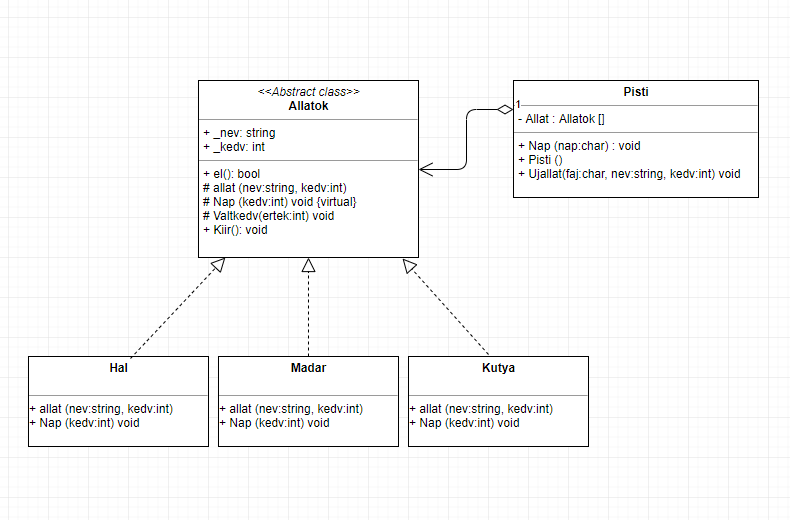
\includegraphics[width=\linewidth]{uml.png}
				\caption{UML}
				\label{fig:uml}
			\end{figure}	
	
	
	\newpage
	\section{Tesztelési terv}	
	\begin{enumerate}
		\item Az állatok alapján
		\begin{enumerate}
			\item A fájl hossza szerint:
			\begin{enumerate}
				\item Üres fájl
				\item Csak egy állat
				\item Sok állat
			\end{enumerate}
		
		\item A fájl eleje és vége szerint:
		\begin{enumerate}		
			\item Első állat éli túl
			\item Első állat hal meg
			\item Utolsó állat éli túl
			\item Utolsó állat hal meg
		\end{enumerate}						
					
		\end{enumerate}
		\item A napok alapján
		\begin{enumerate}
			\item Hossz szerint
			\begin{enumerate}
				\item Egy nap
				\item Sok nap				
			\end{enumerate}
			\item Érték szerint
			\begin{enumerate}
				\item Váltakozó napok
				\item Csak rossz nap, majd csak jó nap	
				\item Csak egy fajta nap							
			\end{enumerate}
		\end{enumerate}		
	\end{enumerate}
		
			
			
			
		
	
		
\end{document}